\documentclass[12pt]{amsart}
%prepared in AMSLaTeX, under LaTeX2e
\addtolength{\oddsidemargin}{-.65in} 
\addtolength{\evensidemargin}{-.65in}
\addtolength{\topmargin}{-.3in}
\addtolength{\textwidth}{1.1in}
\addtolength{\textheight}{.3in}

\renewcommand{\baselinestretch}{1.05}

\usepackage{verbatim,fancyvrb}

\usepackage{palatino}

\usepackage[dvipsnames]{xcolor}

\newtheorem*{thm}{Theorem}
\newtheorem*{defn}{Definition}
\newtheorem*{example}{Example}
\newtheorem*{problem}{Problem}
\newtheorem*{remark}{Remark}

\newcommand{\mtt}{\texttt}
\usepackage{alltt,xspace}
\newcommand{\mfile}[1]
{\medskip\begin{quote}\scriptsize \begin{alltt}\input{#1.m}\end{alltt} \normalsize\end{quote}\medskip}

\usepackage[final]{graphicx}
\newcommand{\mfigure}[1]{\includegraphics[height=2.5in,
width=3.5in]{#1.eps}}
\newcommand{\regfigure}[2]{\includegraphics[height=#2in,
keepaspectratio=true]{#1.eps}}
\newcommand{\widefigure}[3]{\includegraphics[height=#2in,
width=#3in]{#1.eps}}

\usepackage{amssymb}

\usepackage[pdftex, colorlinks=true, plainpages=false, linkcolor=black, citecolor=red, urlcolor=red]{hyperref}

% macros
\newcommand{\bb}{\mathbf{b}}
\newcommand{\br}{\mathbf{r}}
\newcommand{\bv}{\mathbf{v}}
\newcommand{\bx}{\mathbf{x}}
\newcommand{\by}{\mathbf{y}}

\newcommand{\CC}{\mathbb{C}}
\newcommand{\RR}{\mathbb{R}}
\newcommand{\ZZ}{\mathbb{Z}}

\newcommand{\eps}{\epsilon}
\newcommand{\grad}{\nabla}
\newcommand{\lam}{\lambda}
\newcommand{\lap}{\triangle}

\newcommand{\ip}[2]{\ensuremath{\left<#1,#2\right>}}

%\renewcommand{\det}{\operatorname{det}}
\newcommand{\onull}{\operatorname{null}}
\newcommand{\rank}{\operatorname{rank}}
\newcommand{\range}{\operatorname{range}}

\newcommand{\Julia}{\textsc{Julia}\xspace}
\newcommand{\Matlab}{\textsc{Matlab}\xspace}
\newcommand{\Octave}{\textsc{Octave}\xspace}
\newcommand{\Python}{\textsc{Python}\xspace}

\newcommand{\prob}[1]{\bigskip\noindent\textbf{#1.}\quad }

\newcommand{\pts}[1]{(\emph{#1 pts}) }
\newcommand{\epart}[1]{\medskip\noindent\textbf{(#1)}\quad }
\newcommand{\ppart}[1]{\,\textbf{(#1)}\quad }

\newcommand*\circled[1]{\tikz[baseline=(char.base)]{
            \node[shape=ellipse,draw,inner sep=2pt] (char) {#1};}}


\begin{document}
\scriptsize \noindent Math 426 Numerical Analysis (Bueler) \hfill 28 October 2024
\normalsize

\medskip\bigskip

\Large\centerline{\textbf{Assignment \#7}}
\large
\bigskip

\centerline{\textbf{Due Friday, 8 November 2024, at the start of class}}
\medskip
\normalsize

\thispagestyle{empty}

\begin{quote}
{\small
This Assignment is based mostly on Chapter 10 of the textbook,\footnote{Greenbaum \& Chartier, \emph{Numerical Methods: Design, Analysis, and Computer Implementation of Algorithms}, Princeton University Press 2012).} with the exception of problem \textbf{P8} which is from Chapter 8.  Please read all of sections 10.1--10.5.  You can skip sections 10.6 and 10.7.  Reading section 9.2 about Richardson extrapolation would also be a good idea, but I will go over this idea in class; it relates only to Romberg integration in section 10.5.

\medskip
\noindent These expectations always apply to homework:
\renewcommand{\labelenumi}{\arabic{enumi}.\,}
\begin{enumerate}
\item Please put the problems in the order they appear below.
\item When you use \Matlab/etc., show the commands you used along with the results.
\item Please keep a clear distinction between codes, input commands, and computed results and/or figures.
\item Other than the text you write, please minimize use of paper.  For example, computer outputs and figures do not need extra space.
\end{enumerate}
}
\end{quote}

\bigskip
\noindent \textbf{Do these exercises from the textbook:}

\smallskip
\renewcommand{\labelenumi}{{\footnotesize\underline{\textsc{Chapter \arabic{enumi}}}}}
\begin{enumerate}
\setcounter{enumi}{9}
\item ~
    \begin{itemize}
    \item Exercise 2 on page 248
    \item Exercise 3 on page 249
    \item Exercise 6 on page 249
    \end{itemize}
\end{enumerate}

\medskip

\noindent \textbf{Do these additional problems:}

\prob{P8}  \ppart{a}  Trace your hand on a grid and mark 25 to 40 (roughly) equally-spaced points along the trace, and store them into 1D Matlab arrays (i.e.~vectors).  Let $n$ be the number of points.  Here are two ways to do this; pick one:
\begin{itemize}
\item Find/print some grid paper and trace the outline of your hand on it.  Mark the points by hand and enter the $x$ and $y$ coordinates in an editor.
\item Open a big Matlab figure window.  Put your hand on the screen.  Use a Matlab command like \verb|[x,y] = ginput(35)|, and click mouse points.
\end{itemize}

\noindent \begin{minipage}[t]{0.6\textwidth}
The scaling of the grid and/or figure will not matter.  At this point my result looked like the figure at right with $n=36$ points.

\epart{b} Compute and plot the cubic spline interpolant of your data, as a \textbf{parameterized curve} $(x(t),y(t))$.  The indexing of the points can be regarded as $t$-values, namely $t_k=k$ for $k=1,\dots,n$.  The function $x(t)$ interpolates all the pairs $(t_k,x_k)$ and $y(t)$ interpolates all the $(t_k,y_k)$ pairs.  Compute $x(t)$ using the Matlab \texttt{interp1()} function, with the last argument as \texttt{'spline'}.  Do the same thing for $y(t)$.  For plotting you will need to generate a fine grid of $t$ values on the interval $[1,n]$.  Only plot the $(x,y)$ values in the main figure.  Also generate two more figures, smaller is fine,\footnotemark\, for the functions $x(t)$ and $y(t)$.  Make sure to label all axes appropriately.  Other than entering the data for the points $(x_k,y_k)$, your Matlab program should only be a few lines.
\end{minipage}
\begin{minipage}[t]{0.7\textwidth}
\vspace{0pt}

\quad 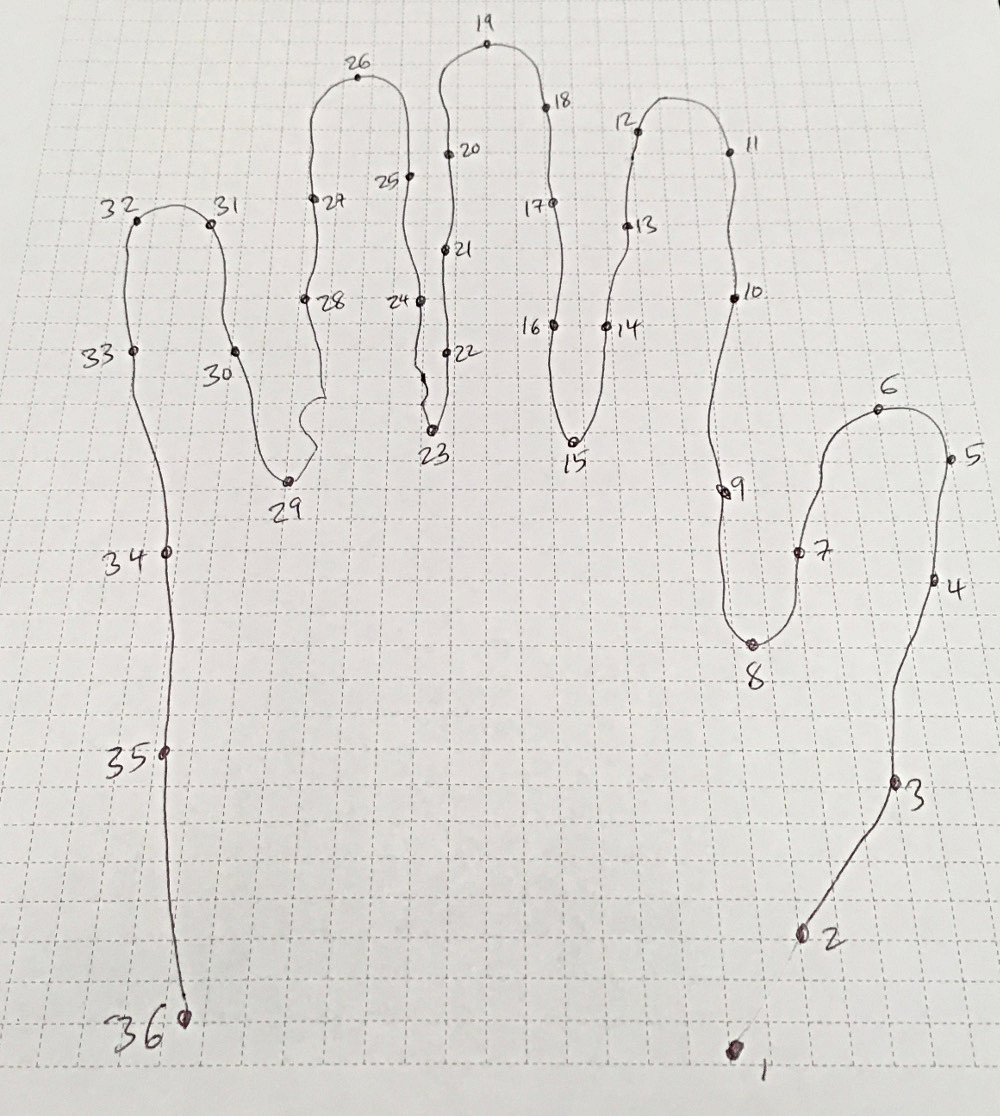
\includegraphics[width=0.6\textwidth]{figs/myhand.jpg}
\end{minipage}
\footnotetext{This is a good application for \texttt{subplot}.}

\prob{P9}  \ppart{a} By using a substitution, compute the exact value of the integral
          $$\int_{-1}^1 x^2 \sin(-5x^3+1)\,dx.$$
Plot the integrand $f(x) = x^2 \sin(-5x^3+1)$ on the interval $[-1,1]$.

\epart{b}  Based on formula (10.6) in Section 10.2, write a composite Simpson's rule code, making it into a convenient function\footnote{My code \texttt{mytrap.m} on the Codes tab is a model for how to write your Simpson's method code.} like
      
       \verb|    z = mysimpsons(f,a,b,n)|

\noindent Using the result from \textbf{(a)}, compute the numerical error when approximating the same integral for $n=10,20,40,80,160,320$ points.  Report this in a small table.

\epart{c}  I posted a very short code called \texttt{clenshawcurtis.m} on the Codes tab.  It is the best possible Matlab implementation of the method described in Section 10.4.  Use it to compute the error when approximating the same integral, again for $n=10,20,40,80,160,320$ points.

\epart{d}  Use \texttt{semilogy} to make a plot of the computed errors for the 2 above methods, in parts \textbf{(b)} and \textbf{(c)}, versus $n$.  That is, put $n$ on the $x$ axis, and the errors on the $y$ axis, with logarithmic scaling of the errors.  Briefly describe what you see, and why it is this way.


\begin{comment}
\prob{P10}  \ppart{a}  Apply my code \texttt{mytrap.m} to try to accurately approximate
          $$\int_0^5 \cos(x^2)\,dx.$$
(I do not know how to find the exact value.)  Use appropriately large values for $n$, and report what you did.  Your goal should be at least 6 correct digits.  How many correct digits do you think you have?

\epart{b}  Implement Romberg integration as described in class, in the form of 
      
       \verb|    [z, count] = myromberg(f,a,b,M)|

\noindent Here \verb|z| is the integral and \verb|count| is the number of function evaluations.  The input \verb|M| is the number of times you double the number of subintervals in the trapezoid rule evaluation.  You may use my code \texttt{mytrap.m}.  You may use \texttt{polyfit} and \texttt{polyval} to do the extrapolation in $h^2$ to $h=0$, or you can follow the book's version on page 243.  Test your implementation on an integral or two where you \emph{do} know the exact answer.

\epart{c}  Now use Romberg integration on the integral in part \textbf{(a)}.  You should be able to get the same (apparent) number of correct digits with far fewer function evaluations.  Report this comparison, accuracy versus number of function evaluations, in a small table.
\end{comment}



\end{document}
